
\begin{procedure}
\item 设置图层。

新建“中心线”和“实线”两个图层,具体设计请参看\ref{sec:dianpian}节的图层设置相关内容。
\item 切换视图为主视图。

\item 绘制中心线,用以辅助绘图。

绘制对称中心线。
\begin{lstlisting}
|命令: XLINE|
|指定点或 [水平(H)/垂直(V)/角度(A)/二等分(B)/偏移(O)]: 52,52|
|指定通过点:$ @1<0$|
|指定通过点:$ @1<90$|
|指定通过点:|
\end{lstlisting}
绘制$\phi 84$中心线圆,其结果如图\ref{fig:dianpiancenterline}所示。
\begin{lstlisting}
|命令: circle|
|指定圆的圆心或 [三点(3P)/两点(2P)/切点、切点、半径(T)]:|
|指定圆的半径或 [直径(D)]: 42|
\end{lstlisting}
\begin{figure}[htbp]
\centering
\begin{floatrow}
\ffigbox{\caption{绘中心线}\label{fig:dianpiancenterline}}{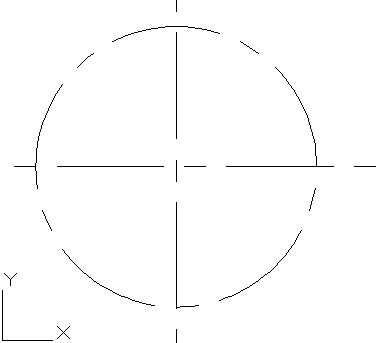
\includegraphics[scale=0.35]{dianpiancenterline.png}}
\ffigbox{\caption{绘$\phi 108$圆柱体}\label{fig:dianpian1}}{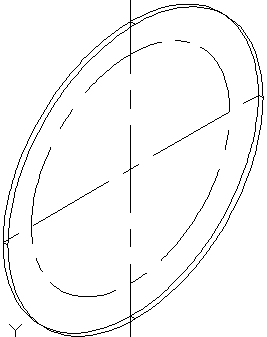
\includegraphics[scale=0.35]{dianpian1.png}}
\end{floatrow}
\end{figure}
\item 切换视图为西南等轴测图。

点击【视图】菜单中【三维视图】子菜单中的【西南等轴测】。
\item 用【圆柱体】命令绘制圆柱体。

【圆柱体】命令的启动方法有:
\begin{itemize}
\item 键盘输入CYLINDER\index{cylinder}或CYL。
\item 【绘图】$\rightarrow$【建模】$\rightarrow$【圆柱体】。
\item 【建模】$\triangleright$【圆柱体】图标
\includegraphics[scale=0.6]{cylinder.png}。
\end{itemize}
绘制$\phi 108$直径的圆柱体,其结果如图\ref{fig:dianpian1}所示。
\begin{lstlisting}
|命令: cylinder|
|指定底面的中心点或 [三点(3P)/两点(2P)/切点、切点、半径(T)/椭|
|圆(E)]:int|
|指定底面半径或 [直径(D)]: 54|
|指定高度或 [两点(2P)/轴端点(A)]$ <2.0000>$: 2|
\end{lstlisting}
绘制$\phi 53$直径的圆柱体,其结果如图\ref{fig:dianpian2}所示。
\begin{lstlisting}
|命令: cylinder|
|指定底面的中心点或 [三点(3P)/两点(2P)/切点、切点、半径(T)/椭|
|圆(E)]:int|
|指定底面半径或 [直径(D)]$ <54.0000>$: 26.5|
|指定高度或 [两点(2P)/轴端点(A)] $<2.0000>$:|
\end{lstlisting}
绘制$\phi 8$直径的圆柱体,其结果如图\ref{fig:dianpian3}所示。
\begin{lstlisting}
|命令: cylinder|
|指定底面的中心点或 [三点(3P)/两点(2P)/切点、切点、半径(T)/椭|
|圆(E)]:int|
|指定底面半径或 [直径(D)] $<26.5000>$: 4|
|指定高度或 [两点(2P)/轴端点(A)]$ <2.0000>$:|
\end{lstlisting}
\begin{figure}[htbp]
\centering
\begin{floatrow}
\ffigbox{\caption{绘$\phi 53$圆柱体}\label{fig:dianpian2}}{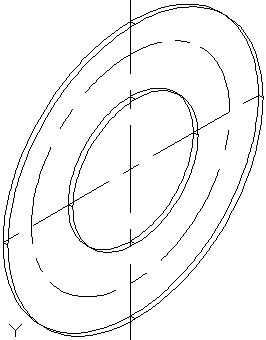
\includegraphics[scale=0.5]{dianpian2.png}}\hspace{30pt}
\ffigbox{\caption{绘$\phi 8$圆柱体}\label{fig:dianpian3}}{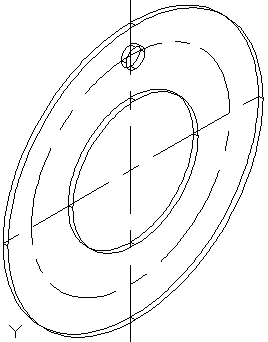
\includegraphics[scale=0.5]{dianpian3.png}}
\end{floatrow}
\end{figure}
\item 关闭“中心线”图层。
\item 三维阵列$\diameter 8$的圆柱,其结果如图\ref{fig:dianpian4}所示。
\newpage
\begin{lstlisting}
|命令: 3darray|
|选择对象: 找到 1 个|
|选择对象:|
|输入阵列类型 [矩形(R)/环形(P)]$<$矩形$>$:p|
|输入阵列中的项目数目: 6|
|指定要填充的角度 (+=逆时针, -=顺时针)$ <360>$:|
|旋转阵列对象? [是(Y)/否(N)] $<Y>$:|
|指定阵列的中心点:|
|指定旋转轴上的第二点:|
\end{lstlisting}
\item 用差集操作完成垫片的三维建模操作。
\begin{lstlisting}
|命令: subtract |
|选择要从中减去的实体、曲面和面域...|
|选择对象: 找到 1 个|
|选择对象:  选择要减去的实体、曲面和面域...|
|选择对象: 找到 1 个|
|选择对象: 找到 1 个,总计 2 个|
|选择对象: 找到 1 个,总计 3 个|
|选择对象: 找到 1 个,总计 4 个|
|选择对象: 找到 1 个,总计 5 个|
|选择对象: 找到 1 个,总计 6 个|
|选择对象: 找到 1 个,总计 7 个|
|选择对象:|
\end{lstlisting}
\begin{figure}[htbp]
\centering
\begin{floatrow}
\ffigbox{\caption{阵列$\phi 8$圆柱体}\label{fig:dianpian4}}{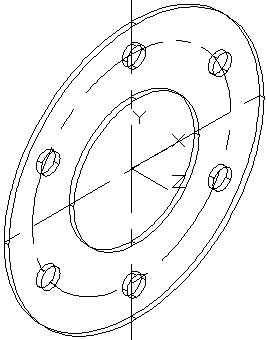
\includegraphics[scale=0.5]{dianpian4.png}}\hspace{30pt}
\ffigbox{\caption{垫片三维模型}\label{fig:dianpian5}}{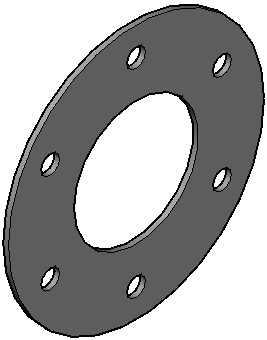
\includegraphics[scale=0.5]{dianpian5.png}}
\end{floatrow}
\end{figure}
\item 设置视觉样式为真实,其结果如图\ref{fig:dianpian5}所示。设置方法为:点击【视图】菜单中【视觉样式】子菜单中的【灰度】项。
\item 将垫片模型保存为“调压阀垫片立体图.dwg”。
\end{procedure}

\endinput